\chapter{Background}
% proposal
\label{ch:background}
In this chapter we present basic concepts that are needed 
to understand better our work. In \autoref{sec:switchedsystems} 
we describe definitions about switched systems and the 
difference between hybrid system a basic concept that we 
will use for our analysis, \cite{sanfelice2020hybrid}. 
In \autoref{sec:safepatterncomputation} we explains the method 
to find patterns. In \autoref{sec:uppaalstratego} we describe 
\textsc{Uppaal Stratego}. In \autoref{sec:onlinestochastichybridcontroller}
 we describe a method to control stochastic hybrid games using online 
 controller. In \autoref{sec:safeandoptimal} we explain the 
 methodology to join the safe and optimal approach. Lastly in 
\autoref{sec:workflow}, we show a general diagram that explain 
how the system works.
\clearpage
  \section{Switched systems}
    \label{sec:switchedsystems}
    \textbf{Switched systems} are loosely defined as dynamical 
    system whose state has two components, one of which evolves 
    in a continuous set such as $\mathbb{R}$  while the other 
    evolves in a discrete set such as $\mathbb{N}$ according to 
    some transition logic based rule. Hybrid System is an abstraction
    of \ac{SS} which is a system which changes acording to switch 
    rule, this rule comprises of discrete events,\citep{branicky1994stability}.    
    \begin{figure}[!hbt]
      \centering
      

\tikzset{every picture/.style={line width=0.75pt}} %set default line width to 0.75pt        

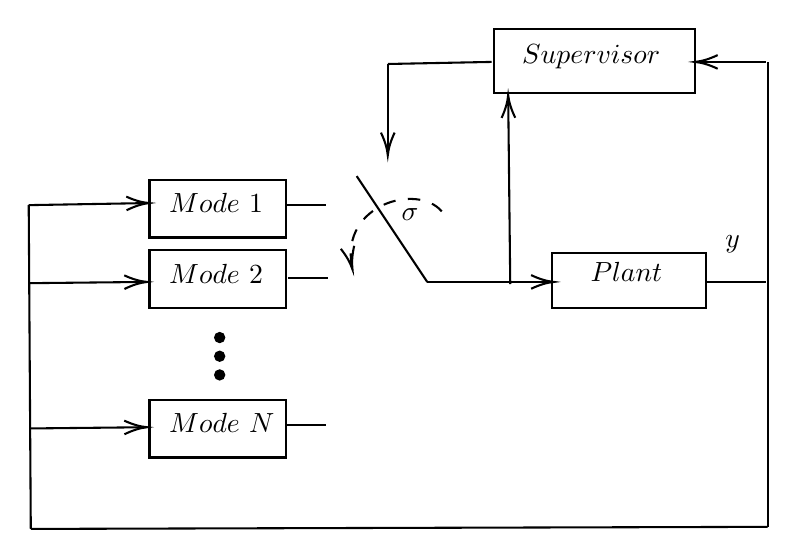
\begin{tikzpicture}[x=0.75pt,y=0.75pt,yscale=-1,xscale=1]
%uncomment if require: \path (0,300); %set diagram left start at 0, and has height of 300

%Shape: Rectangle [id:dp32688849314428636] 
\draw   (190,190.2) -- (255.8,190.2) -- (255.8,218) -- (190,218) -- cycle ;

%Shape: Rectangle [id:dp3126289687771031] 
\draw   (190,118.2) -- (255.8,118.2) -- (255.8,146) -- (190,146) -- cycle ;

%Shape: Rectangle [id:dp46120737421087155] 
\draw   (190,84.2) -- (255.8,84.2) -- (255.8,112) -- (190,112) -- cycle ;

%Shape: Circle [id:dp5034468474397635] 
\draw  [fill={rgb, 255:red, 0; green, 0; blue, 0 }  ,fill opacity=1 ] (221.6,160.2) .. controls (221.6,158.98) and (222.58,158) .. (223.8,158) .. controls (225.02,158) and (226,158.98) .. (226,160.2) .. controls (226,161.42) and (225.02,162.4) .. (223.8,162.4) .. controls (222.58,162.4) and (221.6,161.42) .. (221.6,160.2) -- cycle ;
%Shape: Circle [id:dp7756810170178334] 
\draw  [fill={rgb, 255:red, 0; green, 0; blue, 0 }  ,fill opacity=1 ] (221.6,169.2) .. controls (221.6,167.98) and (222.58,167) .. (223.8,167) .. controls (225.02,167) and (226,167.98) .. (226,169.2) .. controls (226,170.42) and (225.02,171.4) .. (223.8,171.4) .. controls (222.58,171.4) and (221.6,170.42) .. (221.6,169.2) -- cycle ;
%Shape: Circle [id:dp637977438580779] 
\draw  [fill={rgb, 255:red, 0; green, 0; blue, 0 }  ,fill opacity=1 ] (221.6,178.2) .. controls (221.6,176.98) and (222.58,176) .. (223.8,176) .. controls (225.02,176) and (226,176.98) .. (226,178.2) .. controls (226,179.42) and (225.02,180.4) .. (223.8,180.4) .. controls (222.58,180.4) and (221.6,179.42) .. (221.6,178.2) -- cycle ;
%Straight Lines [id:da7143820692778604] 
\draw    (131.8,96.4) -- (187.8,95.43) ;
\draw [shift={(189.8,95.4)}, rotate = 539.01] [color={rgb, 255:red, 0; green, 0; blue, 0 }  ][line width=0.75]    (10.93,-3.29) .. controls (6.95,-1.4) and (3.31,-0.3) .. (0,0) .. controls (3.31,0.3) and (6.95,1.4) .. (10.93,3.29)   ;
%Straight Lines [id:da6291548752080109] 
\draw    (131.8,96.4) -- (132.8,252.4) ;
%Straight Lines [id:da30571480616286983] 
\draw    (132,134) -- (186.8,133.42) ;
\draw [shift={(188.8,133.4)}, rotate = 539.39] [color={rgb, 255:red, 0; green, 0; blue, 0 }  ][line width=0.75]    (10.93,-3.29) .. controls (6.95,-1.4) and (3.31,-0.3) .. (0,0) .. controls (3.31,0.3) and (6.95,1.4) .. (10.93,3.29)   ;
%Straight Lines [id:da5619732357431684] 
\draw    (132,204) -- (186.8,203.42) ;
\draw [shift={(188.8,203.4)}, rotate = 539.39] [color={rgb, 255:red, 0; green, 0; blue, 0 }  ][line width=0.75]    (10.93,-3.29) .. controls (6.95,-1.4) and (3.31,-0.3) .. (0,0) .. controls (3.31,0.3) and (6.95,1.4) .. (10.93,3.29)   ;
%Shape: Rectangle [id:dp825240249219902] 
\draw   (383.8,119.4) -- (458,119.4) -- (458,146) -- (383.8,146) -- cycle ;

%Shape: Rectangle [id:dp9209123444612302] 
\draw   (356,11.4) -- (452.8,11.4) -- (452.8,42.4) -- (356,42.4) -- cycle ;

%Straight Lines [id:da13444253626831282] 
\draw    (304.8,28.4) -- (304.8,70.4) ;
\draw [shift={(304.8,72.4)}, rotate = 270] [color={rgb, 255:red, 0; green, 0; blue, 0 }  ][line width=0.75]    (10.93,-3.29) .. controls (6.95,-1.4) and (3.31,-0.3) .. (0,0) .. controls (3.31,0.3) and (6.95,1.4) .. (10.93,3.29)   ;
%Straight Lines [id:da44360106513864617] 
\draw    (304.8,28.4) -- (354.8,27.4) ;
%Straight Lines [id:da5640561205642627] 
\draw    (289.8,82.4) -- (323.8,133.4) ;
%Straight Lines [id:da987684579468298] 
\draw    (323.8,133.4) -- (382.8,133.4) ;
\draw [shift={(384.8,133.4)}, rotate = 180] [color={rgb, 255:red, 0; green, 0; blue, 0 }  ][line width=0.75]    (10.93,-3.29) .. controls (6.95,-1.4) and (3.31,-0.3) .. (0,0) .. controls (3.31,0.3) and (6.95,1.4) .. (10.93,3.29)   ;
%Straight Lines [id:da6775583049082103] 
\draw    (255.8,96.4) -- (274.8,96.4) ;
%Straight Lines [id:da35489687240032897] 
\draw    (256.8,131.4) -- (275.8,131.4) ;
%Straight Lines [id:da3704670312429943] 
\draw    (255.8,202.4) -- (274.8,202.4) ;
%Straight Lines [id:da7773469448640002] 
\draw    (363.8,134.4) -- (362.82,45.4) ;
\draw [shift={(362.8,43.4)}, rotate = 449.37] [color={rgb, 255:red, 0; green, 0; blue, 0 }  ][line width=0.75]    (10.93,-3.29) .. controls (6.95,-1.4) and (3.31,-0.3) .. (0,0) .. controls (3.31,0.3) and (6.95,1.4) .. (10.93,3.29)   ;
%Straight Lines [id:da6406374988169223] 
\draw    (132.8,252.4) -- (487.8,251.4) ;
%Straight Lines [id:da6415179543064069] 
\draw    (487.8,251.4) -- (487.8,27.4) ;
%Straight Lines [id:da2672609335907974] 
\draw    (486.8,27.4) -- (454.8,27.4) ;
\draw [shift={(452.8,27.4)}, rotate = 360] [color={rgb, 255:red, 0; green, 0; blue, 0 }  ][line width=0.75]    (10.93,-3.29) .. controls (6.95,-1.4) and (3.31,-0.3) .. (0,0) .. controls (3.31,0.3) and (6.95,1.4) .. (10.93,3.29)   ;
%Straight Lines [id:da3287969255166985] 
\draw    (486.8,133.4) -- (458.8,133.4) ;
%Curve Lines [id:da7849132880156575] 
\draw  [dash pattern={on 4.5pt off 4.5pt}]  (330.8,99.4) .. controls (319.04,85.68) and (282.31,95.97) .. (287.43,125.56) ;
\draw [shift={(287.8,127.4)}, rotate = 257.28] [color={rgb, 255:red, 0; green, 0; blue, 0 }  ][line width=0.75]    (10.93,-3.29) .. controls (6.95,-1.4) and (3.31,-0.3) .. (0,0) .. controls (3.31,0.3) and (6.95,1.4) .. (10.93,3.29)   ;

% Text Node
\draw (198,89.4) node [anchor=north west][inner sep=0.75pt]    {$Mode\ 1$};
% Text Node
\draw (198,123.4) node [anchor=north west][inner sep=0.75pt]    {$Mode\ 2$};
% Text Node
\draw (198,195.4) node [anchor=north west][inner sep=0.75pt]    {$Mode\ N$};
% Text Node
\draw (401,122.4) node [anchor=north west][inner sep=0.75pt]    {$Plant$};
% Text Node
\draw (368,17.4) node [anchor=north west][inner sep=0.75pt]    {$Supervisor$};
% Text Node
\draw (310,96.4) node [anchor=north west][inner sep=0.75pt]    {$\sigma $};
% Text Node
\draw (466,109.4) node [anchor=north west][inner sep=0.75pt]    {$y$};


\end{tikzpicture}

      \captionsetup{format=hang}
      \caption{A control diagram of \ac{SS} with a supervisor that determines a switching rule $\sigma$}
      \label{fig:switchedsystem}
    \end{figure}
    \\
    % Let us consider nonlinear switched systems such that  \\
    \textbf{Definition 1.(Hybrid System).} A hybrid system $\mathcal{H}$ is a
    continuous-discrete mathematical abstraction of switched system that represents a 
    tuple $(\tau,\sigma,x,f)$ where defined for all $t \geqslant 0$: \\
    \emph{1. $\tau$ is a time period for switching between modes} \\
    \emph{2. $x \in \mathbb{R}^{M} $ is a vector state of size $M$} \\
    \emph{3. $\sigma \in \mathbb{R}^{N}$ is a vector of $N$ modes that determines a switching rule that will occur at time $\tau,2\tau,..$} depend on time and state ( \ac{SS} only depend on time)\\
    \emph{4. $f$ is a non-linear function subject to a switching rule $\sigma$ and disturbances $d(t)$} \\
    \begin{equation}
        \label{eq:hybridsystem}
        % \dot x(t) = \mathcal{F}_{c,u}(\tau,x(t),d(t)) \\
        % \dot x(t) = f_{\sigma}(x(t),d(t)) \\
        \frac{d}{dt}x(t) = f_{\sigma}(x(t),d(t)) \\
    \end{equation}

    \clearpage
  \section{Online Stochastic Hybrid Controller Synthesis}
    \label{sec:onlinestochastichybridcontroller}
    We use a one-room heating control problem as a running example to 
    demonstrate the technique
    in a simple setting: we model the problem, explain the necessary theory 
    behind the model, show how the model fits the theory and show how 
    \textsc{Uppaal Stratego} can be used to solve the problem.
    The one-room system consists of a room with walls, a window, heater 
    and its controller. The objective of the controller is to maintain 
    the room temperature at the goal level($21 \celsius$). Due to temperature
    sensor energy considerations the controller receives temperature
    readings only once every $15 minutes$ and then it has two options:
    either to turn the heater on (mode "HeatOn") and keep it there or 
    switch the heater off (mode "HeaterOff"). Consequently the temperature 
    evolution will be different in these modes due to different energy 
    supply from the heater. There is also a continuous leak of energy 
    trough the walls and the window to the outside environment. In 
    short, the temperature dynamics can be described by the following 
    differential equation.

    \begin{equation}
        % \dot x(t) = \mathcal{F}_{c,u}(\tau,x(t),d(t)) \\
        \frac{d}{dt}T(t) = (T_e(t)-T(t))A(t)+H(t) \\
    \end{equation}

    Where $T(t)$ is the room temperature at time $t,T_e(t)$ is the 
    outdoor temperature, $A(t)$ is the heat exchange factor specific 
    to the walls and windows, and $H(t)$ is the power of the heater.
  
    \begin{figure}[!htb]
      \begin{subfigure}{0.60\textwidth}
        \centering
        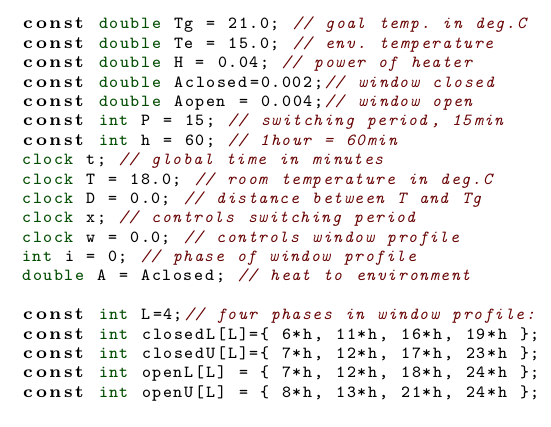
\includegraphics[width=\linewidth]{images/oneroom1.png}
        \caption{Variable declarations.} \label{fig:1a}
      \end{subfigure}
      \hspace*{\fill}
      \begin{subfigure}{0.35\textwidth}
          \begin{subfigure}{\textwidth}
            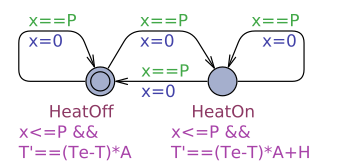
\includegraphics[width=\linewidth]{images/heatingmodes.png}
            \caption{Heating modes.} \label{fig:1b}
          \end{subfigure}
        % \hspace*{\fill}
          \begin{subfigure}{\textwidth}
            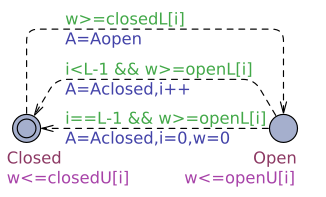
\includegraphics[width=\linewidth]{images/windowprofile.png}
            \caption{Window profile.} \label{fig:1c}
          \end{subfigure}
          % \hspace*{\fill}
          \begin{subfigure}{\textwidth}
            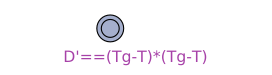
\includegraphics[width=\linewidth]{images/distancetogoal.png}
            \caption{Distance to goal temp.} \label{fig:1d}
          \end{subfigure}     

      \end{subfigure}
      
      \caption{\textsc{Uppaal Stratego} model of one room with one window}
    \end{figure}

    \autoref{fig:1b} shows such differential equation with heater step functions 
    modelled in \textsc{Uppaal Stratego} as hybrid automaton with two discrete 
    modes. The continuous dynamics of $T(t)$ is typeset as an invariant constraint over the 
    clock variable $T$ derivative under the respective modes. The periodic 
    behaviour of the controller is enforced by the invariant $x<=P$ and the guard $x==P$
    over clock $x$ with default derivative of 1. For the sake of simplicity,
    we assume static outdoor temperature fixed to a specific value and 
    modelled by the constant floating point variable $Te$. All model v
    variables (their types and initial values) are declared as $C$ structures
    in \autoref{fig:1a}. The window step function $A(t)$ is modelled In
    \autoref{fig:1c} as stochastic automaton with transitions between "Open"
    and "Closed" modes and changing the floating point variable $A$. Thus
    the window process can change the value of $A$ discretely between values
    \textbf{Aclosed} and \textbf{Aopen} at any moment with uniform probability 
    distribution over time, but only at intervals specified by a user 
    profile. The profile is stored in arrays \textbf{closedL/U} and \textbf{openL/U}
    denoting the lower and upper bounds of time intervals when the switch 
    may happen. For example, one can read the profile arrays by columns:
    the window starts and stays closed during the night time, but it will 
    open somewhere between 6 and 7 o'clock in the morning and close between
    12 and 13, etc. 

    The whole system model is then a composition of the controlled heating 
    process with the stochatic window process where temperature depends on 
    the heating mode and the mode of the window. We use stochastic hybrid 
    game to describe the controller synthesis formally.






    \textbf{Definition 2.(Stochastic Hybrid Game).} A stochastic hybrid game $\mathcal{G}$ is a
    tuple $(\mathcal{C,U,X,F},\delta)$ where:
    \\
    \\
    \emph{1. $\mathcal{C}$ is a controller with a finite set of (controllable) modes C.} \\
    \emph{2. $\mathcal{U}$ is the environment with a finite set of (uncontrollable) modes U.} \\
    \emph{3. $\mathcal{X} = \left\lbrace x_1,x_2,..x_n \right\rbrace$ is a finite set of
    continuous (real-valued) variables } \\
    \emph{4. for each c $\in$ C and $u \in U, \mathcal{F}_{c,u} : \mathbb{R}_{>0}
      \times \mathbb{R}^X \rightarrow\mathbb{R}^X$ 
        is the flow-function that describes the evolution of the continuous variables
        over time in the combined mode (c,u), and} \\
    \emph{5. $\delta$ is a family of density functions, $\delta_\gamma: 
    U \rightarrow 
    %\mathbb{R}_{\geqslant 0} \times U \rightarrow 
    [0,1]$, where $ \gamma = (c,u,v) \in C \times U
    %\mathbb{R}_{\geqslant 0}$, where $ \gamma = (c,u,v) \in C \times U
    \times \mathbb{R}^X$ is a global configuration.
    More precisely, $\delta_{\gamma}(u')$ is the probability that $u \in \mathcal{U}$
    in the global configuration $ \gamma = (c,u,x)$ will change to the
      uncontrollable mode $u'$ after a delay of $\tau$ 
      \footnote{Note that $\sum_u,\int_{\tau}\delta_{c,u,v}(\tau,u')d\tau = 1$ for all $(c,u,v)$.}}.

    We shall assume that among the continuous variables $\mathcal{X}$, there is a variable
    \textbf{time} measuring global time, i.e $\mathcal{F}_{c,u}(\tau,v)(\textbf{time})$ 
    for any mode-configuration $(c,u)$. In the above definition, the syntatic specification
    of flow functions---e.g. using ODEs---has been left open. In the game $\mathcal{G}$,
    the controller $\mathbb{C}$ will only be permitted to change controllable mode at time-points
    being a multiple of some given period $P$ (hence the term switched control). In contrast,
    the environment $\mathbb{U}$ will change its uncontrollable mode according to the 
    family of density function $\delta_\gamma$.
    
  

    \emph{Example 1}. In our one-room example, the controllable modes are {\color{RawSienna} HeatOff}
    and {\color{RawSienna} HeatOn} with controllable transitions (using solid lines) between
    them, the uncontrollable are {\color{RawSienna} Open} and {\color{RawSienna} Closed} with
    uncontrollable transitions (using dashed lines). We also have a number of continuous 
    variables: temperature T and clocks t,x and w. The differential equations together with
    discretely changing variables are part of the flow-functions definition.

    Now let $\mathbb{C}$ denote the set of global configurations $C\times U \times \mathcal{R}^X$
    of the game $\mathbb{G}$. Then a (memoryless) strategy $\sigma$ for the controller $\mathcal{C}$
    is a function $\sigma: \mathbb{C} \rightarrow C$, i.e. given the current
    configuration $\gamma = (c,u,v)$, the epression $\sigma(\gamma)$ is the controllable mode
    to be used in the next period.

    Let $\gamma = (c,u,v)$ and $\gamma' = (c',u',v')$. We write $\gamma \xrightarrow{\tau} \gamma'$ 
    in case $c'=c, u'=u$ and $v'=\mathcal{F}_{(c,u)}(\tau,v)$. We 
    write $\gamma \xrightarrow{\tau}_{u} \gamma'$ in case $c'=c, v'=\mathcal{F}_{(c,u)}(\tau,v)$
    and $\delta_{\gamma}(\tau,u') > 0$. Let $\sigma: \mathbb{C} \rightarrow C$
    be a (memoryless) strategy. Consider an interleaved sequence $\pi$ of configurations and
    relative time-delays of the form:
    
    \begin{center}
      $\pi = \gamma_0 :: \tau_1 :: \gamma_1 :: \tau_2 :: \lambda_2 :: \tau_3 :: \gamma_3 ...$  
    \end{center}

    where $\gamma_i = (c_i,u_i,v_i), \tau_i \in \mathbb{R}_{\geqslant 0}$ and for all \emph{n} 
    there  exist \emph{i} st. $\sum_{j \geqslant i}\tau_j = nP$. Then $\pi$ is a run according
    to the strategy $\sigma$ if for all \emph{i} either $\gamma_i \xrightarrow{\tau_{i+1}}u \gamma_{i+1}$
    or $\sum_{j \geqslant i+1}\tau_j$ is multiple of P and $\gamma_i \xrightarrow{\tau_{i+1}} (c_i,u_i,v_{i+1})$
    with $c_{i+1} = \sigma(c_i,u_i,v_{i+1})$ and $u_{i+1}=u_i$.

    In fact, under a given strategy $\sigma$ of the game $\mathcal{G}$ becomes a completly 
    stochastic process $\mathcal{G}|\sigma$, inducing a probability measure on sets of runs.
    Thus, if $H \in \mathbb{N}$ is a given time-horizon, and $D$ is a random variable on runs--e.g.
    measuring the integrated deviation of the continuous variables wrt. given target values--
    then $\mathbb{E}^{\mathcal{G,\gamma}}_{\sigma,H}(D) \in \mathbb{R}_{\geqslant 0}$ is 
    the expected value of $D$ with respect to random runs of $\mathcal{G}|\sigma$ of length
    $H$ starting in the configuration $\gamma$. We want to obtain a strategy $\sigma^H$ which
    minimizes (or maximizes) this expected value.


  \section{Uppaal Stratego}     
    \label{sec:uppaalstratego}
      We use the modelling tool \textsc{Uppaal Stratego} for control 
      synthesis. It integrates \textsc{Uppaal} with the two branches
      \textsc{Uppaal SMC}(statistical model checking for stochastic 
      hybrid systems) and \textsc{Uppaal Tiga} (synthesis for timed games).
      Therefore, \textsc{Uppaal} is able to synthetize safe and
      optimal strategy $\sigma_{opt}$. We use Dynbex and safe algorithms
      first we abstract the \ac{SHG} ignoring all stochasticity.
      Subsequently, reinforcement learning is used to obtain an 
      optimal sub-strategy $\sigma_{opt}$ based on $\mathcal{G}|
      \sigma_{safe}$ and the given random optimization variable.
      Several learning algorithms are at the modelers disposal in 
      \textsc{Uppaal Stratego}. Recently, 

      \textsc{Uppaal Stratego} offers four learning methods focusing on various parts of the model,
      therefore we consider the quality and the cost of each method before we focus on our 
      industrial-scale example. \textbf{Table} shows a summary of the evaluation of various 
      methods on two variants of a one-room example: the purely dynamical model is show in \textbf{Fig1}
      and another one that has an extra counter incremented at each period $P$. The result
      is that among that offline methods (discussed so far) the "splitting" method provides 
      the smallest distance solution, however it is costlier than others in \textbf{CPU} time
      and memory. The right side \textbf{Table} shows that if we add a period counter to our
      model, then other methods dominate and the "splitting" method is no longer as good and 
      the "naive" computation costs significantly less. Offline-6 section (strategy for six days)
      requires twice as many resources as offline-3 (strategy for three days) which means 
      that a linear number of resources is needed in terms of duration of the strategy while 
      using the same number of runs, but the quality (distance) degraded almost four times
      with a period counter. 
  
      \begin{figure}[!hbt]
        \centering
        
\includegraphics[width=0.4\linewidth]{images/uppaalstratego.jpeg}
        \captionsetup{format=hang}
        \caption{ \textsc{Uppaal Stratego}, facilitates generation, optimization, comparison as well as consequence and performance exploration of strategies for stochastic priced timed games in a user-friendly manner.}
        \label{fig:uppaalstratego}
      \end{figure}

      
    \emph{Example 2.} The one-room controller's goal is to keep the room temperature as 
    close as possible to the goal set point, therefore a desired controller would minimize 
    the absolute difference $T(t)-T_g$. In order to encourage the minimization even more
    we use a quadratic difference function to measure the distance between the room $T$ 
    and the goal $T_g$ temparatures, and then integrate it to achieve a distance function 
    over complete trajectories. Conveniently, our distance function is modelled using 
    differential equation in \autoref{fig:1d} as a separate process. Before we synthetize anything,
    we can inspect how does a uniform random choice fare in \emph{fig}: the temparature curve 
    is at the top and heating and window  mode trajectories are bellow and they jump up
    when the heating is on the window is open respectively. The result is that the room 
    temperature responds to the mode changes and varies widely, tending to overshoot above the
    goal, and hence the distance function after $24h$ period is about 4200 on average. In order
    to synthetize a strategy we pose the following query in \textsc{Uppaal Stratego}:

    \begin{lstlisting}[language=Octave]
        strategy opt = minE (D) [<=24h]: <> t==24*h
    \end{lstlisting}

    which asks to find the strategy that will minimize the expected value of $D$ when we reach
    a state with $t == 24*h$ while considering simulations of up to $24*h$ in duration. Once
    the strategy is available, we may inspect it by requesting a simulation plot:

    \begin{lstlisting}[language=Octave]
        simulate 1 [<=24*h]{T, Window.Open+14, Room.HeatOn+16} under opt
    \end{lstlisting}

    For example, the synthetized 24h strategy using the "naive" learning method yields
    the distance od 2750 on average as shown in \emph{Fig}. The result is even more improved
    by  the "splitting" learning method in \emph{Fig} where the temperature oscillates around
    the goal very closely.    

    

    \clearpage

    \begin{figure}[!htb]
        \begin{subfigure}{0.51\textwidth}
            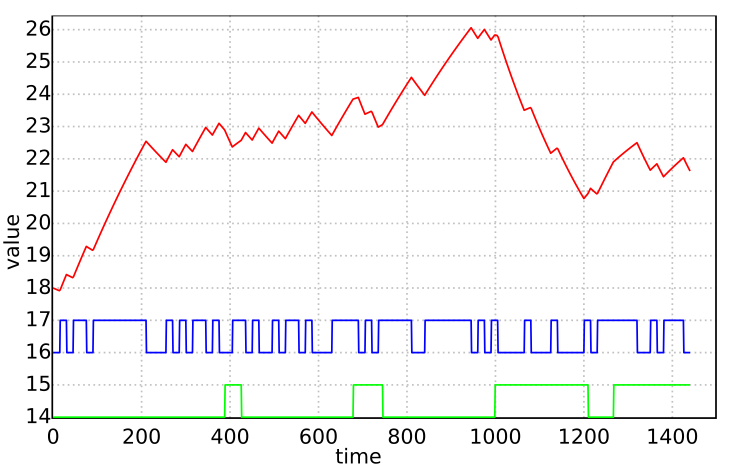
\includegraphics[width=\linewidth]{images/2_a.png}
            \caption{Stochastic, $D(24h)=4200$.} \label{fig:2a}
        \end{subfigure}%
        \hspace*{\fill}
        \begin{subfigure}{0.51\textwidth}
            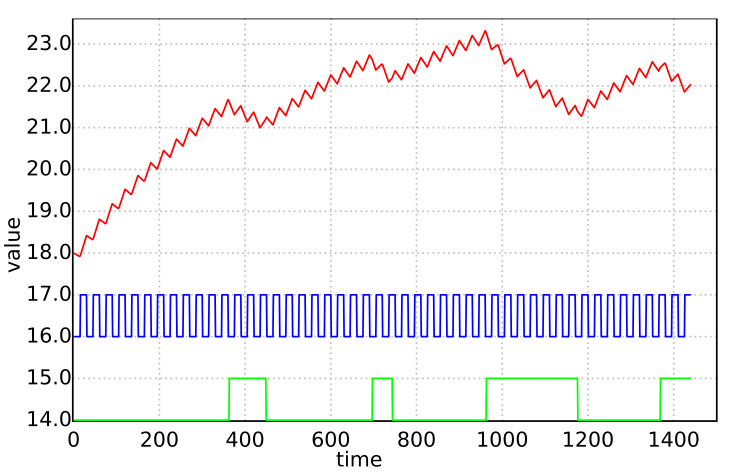
\includegraphics[width=\linewidth]{images/2_b.png}
            \caption{Offline naive. $D(24h)=2750$.} \label{fig:2b}
        \end{subfigure}%    
        \\
        \begin{subfigure}{0.51\textwidth}
            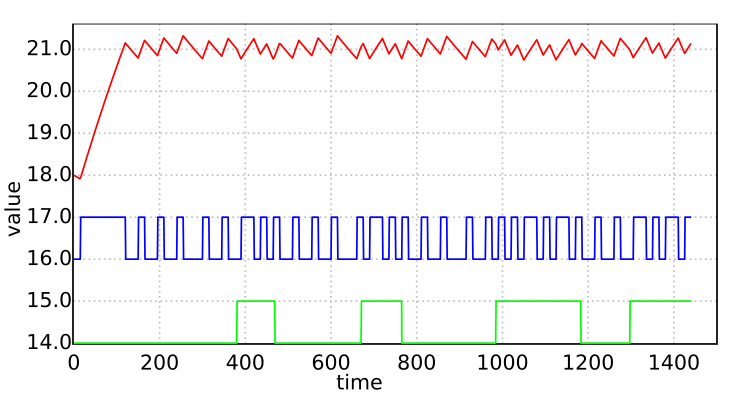
\includegraphics[width=\linewidth]{images/2_c.png}
            \caption{Offline splitting, $D(24h)=468$.} \label{fig:2c}
        \end{subfigure}%
        \hspace*{\fill} 
        \begin{subfigure}{0.51\textwidth}
            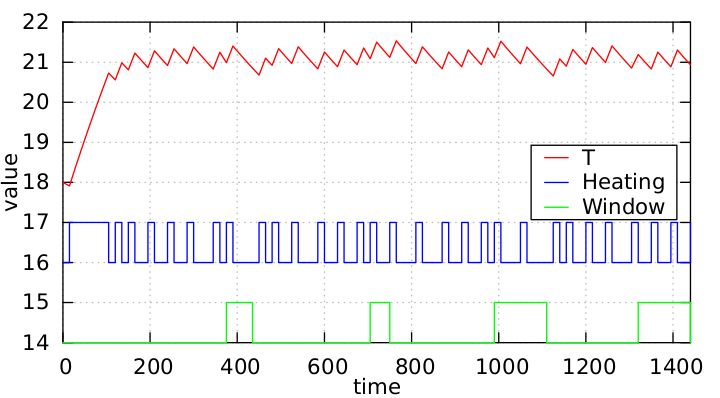
\includegraphics[width=\linewidth]{images/2_d.png}
            \caption{Online naive, $D(24h)=471.5$.} \label{fig:2d}
        \end{subfigure}%
        \caption{One-room 24h trajectories of various control strategies}
    \end{figure}

    % \textbf{Online Synthesis}
  \section{Online Synthesis}
    \textsc{Uppaal Stratego} [5,6] provides a method for aproximating 
    $\mathbb{E}^{\mathcal{G},\gamma}_{\sigma,H}(D) \in \mathbb{R}_{\geqslant 0}$
    by computing a near-optimal strategy $\sigma^H$ for a given horizon $H$ using 
    reinforcement learning. However, the effort needed to learn the strategy  
    $\sigma^H$ with a desired precision and confidence-level grows exponentially
    in the number of dimensions (variables). The quality of the learned control 
    degrades sharply after the control options outnumber the number of simulation
    runs during learning, making this direct application of \textsc{Uppaal Stratego}
    limited in the time horizon. For instance, given a realistic setting of eleven 
    heating switches as considered in our case study, the controller is faced with  
    $2^11=2048$ distinct options at each 15min period and thus \textsc{Uppaal Stratego}
    manages to compute sensible heating configuration only for the first two periods 
    (yieldings $2048^2=4194304$ combinations in total) and then it simply resolves 
    to default option of no heating at all.
    Instead of learning --- at great computational expense -- the   entire strategy
    $\sigma^H$, we propose a method for attentively and online (i.e while playing
    the game $\mathcal{G}$ in the real setting) to compute a near-optimal strategy for 
    controllable mode-change at the next period. More precisely, the resulting online 
    and periodic strategy $\sigma^O$ will base the mode-change at time $nP$ not only
    on the configuration at that point ($\gamma_n$) but also on the configuration
    ($\gamma_{n-1}$) at time $(n-1)P$\footnote{Note that there way be several configurations
    between $\gamma_{n-1}$ and $\gamma_n$ due to the environment $\mathcal{U}$ changing
    the uncontrollable mode.}, which will be used as the basis for online
    learning of short-horizon $(h << H)$ strategies.

    \begin{table}[H]
    \caption{Performance evaluation of one room controller synthesis: offline-3(-6) methods
        synthetize strategy for entire 72 hours (144 hours respectively ) at once,
        strategy distance is evaluated on 70 simulations; online-3 methods synthetize
        a strategy for 5 periods of 15 min ahead and repeat synthesis and execution until 
        72 hours are covered, the distance is averaged over 70 online simulations.
    }


    \centering
    \begin{tabular}{|c|l|r|r|r|r|r|r|}
    \hline
    % \parbox[t]{2mm}{\multirow{2}{*}{Synthesis method}}
    & \multirow{2}{*}{ \textbf{\pbox{10cm}{Synthesis \\ method}} } & \multicolumn{3}{c|}{ \textbf{Purely dynamical model} } & \multicolumn{3}{c|}{ \textbf{Extra period counter} } \\
    % \hline
    & & \multicolumn{1}{c|}{ \textbf{Distance} } & \multicolumn{1}{c|}{ \textbf{cpu,s} } & \multicolumn{1}{c|}{ \textbf{mem,kB}} & \multicolumn{1}{c|}{ \textbf{Distance} } & \multicolumn{1}{c|}{ \textbf{cpu,s} } & \multicolumn{1}{c|}{ \textbf{mem,kB} } \\
    \hline
    \bfseries \parbox[t]{2mm}{\multirow{4}{*}{\rotatebox[origin=c]{90}{Offline-3}}}
    & naive & 10227.8 & 1555.15& 11884& 3671.84 & 566.4 & 9448 \\
    & splitting & 517.9 & 1640.06 & 13424& 2361.80 & 1608.48 & 90740\\
    & covariance & 10227.8 & 1298.66& 11896& 1091.81 & 1668.45 & 22820 \\
    & regression & 10227.8 & 1368.34 & 11480& 1387.84 & 1767.50 & 19196 \\
    \hline
    \bfseries \parbox[t]{2mm}{\multirow{4}{*}{\rotatebox[origin=c]{90}{Offline-6}}}
    & naive & 19668.8 & 1855.36 & 11836 & 8032.86 & 1316.08 & 20820\\
    & splitting & 593.7 & 3200.38 & 13112 & 8260.19 & 3120.03 & 167308 \\
    & covariance & 20234.3 & 2039.30 & 11528 & 2468.91 & 3258.09 & 39580 \\
    & regression & 19007.2 & 2525.13 & 12148 & 3425.62 &  3488.26 & 28416 \\
    \hline
    % ±
    \bfseries \parbox[t]{2mm}{\multirow{4}{*}{\rotatebox[origin=c]{90}{Online-3}}}
    & naive & 584.7$\pm$1.0 & 1046.5$\pm$5.0 & 7240 & 526.6$\pm$0.5 & 1227.1$\pm$3.2 & 7328 \\
    & splitting & 547.7$\pm$0.6 & 1136.4$\pm$3.6 & 7384 & 526.1$\pm$0.6 & 1240.8$\pm$2.5 & 7384 \\
    & covariance & 587.5$\pm$1.2 & 1084.0$\pm$3.9 & 7272 & 527.1$\pm$0.6 & 1158.5$\pm$2.5 & 7624 \\
    & regression & 585.3$\pm$1.0 & 1173.9$\pm$3.4 & 9052 & 527.9$\pm$0.5 & 1337.1$\pm$2.5 & 7380 \\
    \hline
    \end{tabular}
    \label{table:t1}
    \end{table}

    Formally:
    \begin{equation*}
        \sigma^O (\gamma_{n-1},\gamma_{n}) =^{\text{def}} \textbf{let}(\sigma^h = \textbf{argmin}_{\sigma}\mathbb{E}^{\mathcal{G},\gamma_{n-1}}_{\sigma,h}(D) ) \textbf{ in } \sigma^h(\gamma_n) 
    \end{equation*}

    We leave the formal definition of runs under the one-step-memory strategy $\sigma^O$
    to the reader (slightly more complicated version of runs under a memoryless strategy given above).
    However, we note that $\sigma^O$ may be used for an arbitrary finite horizon $H$ or 
    even as a strategy of infinite horizon. To maximize the quality of $\sigma^O$, the choice
    of the small horizon $h$ should be such that it just allows the learning of $\sigma^h$
    to be completed between the two configurations $\gamma_{n-1}$ and $\gamma_n$, i.e.
    within the period $P$.  

    \emph{Example 3}. We implemented the online strategy evaluation on the one-room 
    example by repeatedly calling \textsc{Uppaal Stratego} to synthetize 
    and evaluate the computed strategy. The following steps are involved:
    
    \begin{enumerate}
      \item Synthetize a strategy capable of adapting for 5 periods ahead where 
      \textbf{LastTime} starts with 0: \textbf{ \text{strategy S = minE(D) [<= 5*P]: <> == LastTime+5*p}}
      \item Simulate the system for 1 period using the strategy S and record its Last
      state: \textbf{ \text{simulate 1 [<=P] { t, T, Room.HeatOn, x, Window.Open, w, i, D }}}
      \item Create a copy of the original model and replace the initial state with the 
      recorded state from the simulation above.
      \item Increment \textbf{\text{LastTime}} by $P$ and repeat the synthesis and 
      simulation from step 1 until a required number of periods is simulated.
      \item Record the final value of the distance variable $D$.
    \end{enumerate}    

    The short trajectories from step 2 are then switched together to produce 
    a continuous trajectory of the entire 3 day simulation. An example result of 
    the first $24h$ is displayed in \autoref{fig:2d} which is also comparable 
    to other strategies. The online-3 section \autoref{table:t1} shows the averages
    of the recorded distances together with the overall synthesis effort for 
    entire 3 day emulation. The encouraging result is that the short strategy 
    synthesis takes only 4-8 seconds and the overall quality of any online 
    synthesis method is very close to the best and expensive offline-3 outcome 
    (the offline "splitting" method).


  \section{Safe patterns computation}
  \label{sec:safepatterncomputation}
    In this part is presented some definitions based on an existing 
    procedure of state-space bisection and made available for nonlinear 
    systems  with the help of guaranteed integration, the algorithm has
    been  improved to be able to consider longer patterns of modes with a better
    pruning approach. The method consist of given a objective region 
    \emph{R}, a set \emph{S} and a forbidden reigion \emph{B}, the method find a pattern $\pi_i$, $i \in 
    \mathbb{N}$. \cite{le2016distributed}

    % \textbf{Problem 1} (Control Safe Synthesis). Let us consider a 
    % hybrid system as defined in \autoref{eq:hybridsystem}. Given 
    % three sets R, S and B 
    
    
  
    \textbf{Definition 3}\emph{(Safe Control Synthesis)}. Let us 
    consider a hybrid system defined in \autoref{eq:hybridsystem}. Given three sets R, S and B, 
    with ${R \cup B \in S}$  and ${R \cap B = \varnothing }$. % find a 
    The system is safe if there is a rule ${\sigma : \mathbb{R}^+ \rightarrow U}$ such that, 
    for any ${x_0 \in R }$ and any perturbation $p : \mathbb{R}^+ \rightarrow U$
    the following holds: 

    \begin{itemize}
        \item \emph{ ${\tau}$-stability: ${x(t)}$ return in R 
        infinitely often, at some multiples of sampling time ${\tau}$}.
        \begin{equation}
          \forall k \in \mathbb{N}, x(k\tau, t_0,x_0,\sigma,w) \in R
        \end{equation}
        \item \emph{ safety: ${x(t)}$ always stays in ${S/B}$.}        
        \begin{equation}
          \forall t \in \mathbb{R}, x(t, t_0,x_0,\sigma,w) \in S, \
          x(t, t_0,x_0,\sigma,w) \notin B
        \end{equation}
    \end{itemize}

    \textbf{Definition 4}(Inclusion function). \emph{Consider a function 
    $f :\mathbb{R}^n \rightarrow \mathbb{R}^m$, then $[f]:\mathbb{R}^n \rightarrow \mathbb{R}^m$}
    is said to be an extension of f to intervals if
    \begin{eqnarray*}
      \forall [x] \in \mathbb{R}, [f]([x]) \subseteq {f(x), x \in [x]}.      
    \end{eqnarray*}

    It is possible to define inclusion functions for all elementary 
    functions such as x,sin,cos,exp, and so on. The \emph{natural}
    inclusion function is the simplest to obtain: all occurrences 
    of the real variables are replaced by their interval counterpart
    and all arithmetic operations are evaluated using interval 
    arithmetic. More sophisticated inclusion functions such as the 
    centered form, or the taylor inclusion function may also be used.
    We now introduce the Initial 

    One of main features of this approach is the Initial Value Problem, 
    which is introduced as follow:

    \textbf{Definition 5} Initial Value Problem(IVP). Consider an ODE 
    with a given initial condition.
    \begin{eqnarray*}            
      \label{eq:ivp}      
      \dot{x} = f_{\sigma(t)}(x(t),d(t)), \\ 
      with, x(0) \in X_0, d(t) \in [d],  \\
    \end{eqnarray*}
    with $f:\mathbb{R}^+ \times \mathbb{R}^n \times \mathbb{R}^m \rightarrow \mathbb{R}^n $
    assumed to be continuous in $t$ and $d$ and globally Lipschitz in $x$. we
    assume that parameters $d$ are bounded (used to represent the disturbance).
    An IVP consists in finding a function $x(t)$ described by \autoref{eq:ivp}
    for all $d(t)$ lying in $[d]$ and for all the initial conditions in $X_0$.
    
    \textbf{Definition 6} Let $X \in \mathbb{R}^n$ be a box of the state
    space. Let $\pi = (i_1,i_2,..,i_k) \in U^k$. The successor set of $X$
    via $\pi$, denoted by $Post_{\pi}(X)$, is the (over-approximation of the)
    images of $X$ induced by application of the pattern $\pi$, i.e, the 
    solution at time $t=k\tau$ of 
    \begin{eqnarray*}
      \dot{x} = f_{\sigma(t)}(x(t),d(t)), \\
      x(0) = x_0 \in X, \\
      \forall t \geqslant 0, d(t) \in [d], \\
      \forall j \in \lbrace 1,..,k \rbrace, \sigma(t) = i_j \in U \text{ for } t \in [(j-1)\tau,j\tau>
    \end{eqnarray*}
    
    \textbf{Definition 7} Let $X \in \mathbb{R}^n$ be a box of the state
    space. Let $\pi = (i_1,i_2,..,i_k) \in U^k$. We denote by $Tube_{\pi}(X)$4
    the union  of boxes covering the trajectories of IVP, whose construction 
    is detailed in 
    
    \textbf{Remark 1}. $Post_{\pi}(X)$ is an over-approximation at time 
    $ t=k\tau $ of the set of states originated from the set $X$ 
    at time $t=0$, while $Tube_{\pi}(X)$ is an over-approximation
    of the whole set of states between $t=0$ and $t=k\tau$ originated
    from the set $X$ at time $t=0$.

    \begin{algorithm}    
        \caption{Decomposition}\label{decomposition}    
        \begin{algorithmic}[1]
          \Procedure{Decomposition}{$W,R,S,B,D,K$}\Comment{List of set of patterns} \\
            \textbf{Input:} A box $W$, a box $R$, 
            a box $S$, a box $B$, a degree $D$ of bisection, a length $K$ of input pattern\\
            \textbf{Output:} $ \lbrace(V_i,\pi_i)\rbrace_i, True $ or $ <_,False>$ \\          
            $(\pi,b) := FindPattern(W,R,S,B,K)$
            \If{ $b = True$}
              \State return $<\lbrace (W,pat) \rbrace,True>$
            \Else
              \If{ $D = 0$}
                \State return $<,False>$
              \Else
                \State Divide equally $W$ into $(W_1,W_2)$
                \For{ $i=1,2$}
                  \State $(,b_i) = Decomposition(W,R,SB,D-1,K)$
                \EndFor
              \EndIf
            \EndIf
            \State \textbf{return} $<_,False>$.
          \EndProcedure    
        \end{algorithmic}
      \end{algorithm}


      \begin{algorithm}
        \caption{Find Pattern}\label{findPattern}
        \begin{algorithmic}[1]
          \Procedure{FindPattern}{$W,R,S,B,K$}\Comment{List of set of patterns} \\
            \textbf{Input:} A box $W$, a box $R$,
            a box $S$, a box $B$, a length $K$ of input pattern\\
            \textbf{Output:} $<\prod,True> or <_,False>$ \\
            $\mathcal{S}= \lbrace \emptyset \rbrace$ \\
            $\mathcal{L}= \lbrace (W,W,\emptyset) \rbrace$
            \While{$\mathcal{L} \neq \emptyset$}
              \State $e_{current} = takeHead(\mathcal{L})$
              \For{$i \in U$}:
                \If {$ Post_{i}(e_{current}.Y_{current}) \subseteq R$ \textbf{and} $Tube_{i}(e_{current}.Y_{current}) \cup B = \emptyset $ \textbf{and} $Tube_{i}(e_{current}.Y_{current}) \cup B \subseteq S $ }
                  \State putTail($\mathcal{S}e_{current}.\prod + i$)
                \Else
                  \If{$ Tube_{i}(e_{current}.Y_{current}) \cap B \neq \emptyset $ \textbf{or} $ Tube_{i}(e_{current}.Y_{current}) \nsubseteq S $}
                    \State discard $e_{current}$
                  \EndIf
                  \If{$ Tube_{i}(e_{current}.Y_{current}) \cap B = \emptyset $ \textbf{and} $ Tube_{i}(e_{current}.Y_{current}) \subseteq S $}
                    \If {$Length(\prod)+1<K$}
                      \State putTail$(\mathcal{L},(e_{current}.Y_{init}.Post_{i}(e_{current}.Y_{current}),e_{current}.\prod+i))$
                    \EndIf              
                  \EndIf
                \EndIf
              \EndFor
            \EndWhile
            \State \textbf{return} $<_,False>$ \Comment{if no solution is found, or $<\prod,True>$, $\prod$ beaing any pattern validated in $Solution$.}
          \EndProcedure    
        \end{algorithmic}
      \end{algorithm}
    \clearpage



  \section{Safe and optimal strategies for stochastic hybrid games}
    \label{sec:safeandoptimal}
    For a given \ac{SHG}, a nondeterministic \emph{strategy} $\sigma$.
    Formally, a strategy is a function $\sigma: \mathbb{C} \rightarrow 2^C$
    ,where we denote $\mathbb{C}$ the set of global configurations 
    $\gamma = (c,u,x) \in C \times U \times \mathbb{R}^X$
    that returns a nonempty set of allowed modes in a configuration  
    $\gamma$.
    % 20
    The behavior of the \ac{SHG} $\mathcal{G}$ under supervision of a 
    strategy $\sigma$, denoted as the stochastic process $\mathcal{G}|\sigma$,
    is defined as follows. A run $\pi$ of \ac{SHG} is an interleaved 
    sequene $\pi \in \mathbb{C} \times (\mathbb{R}_{\geqslant 0} 
    \times \mathbb{C})^{*}$ of configurations and time-delays of 
    some given period $P$, starting with initial configuration $\gamma_0$: 
    \begin{center}
      $\pi = \gamma_0 :: P :: \gamma_1 :: P :: \gamma_2 :: P :: \gamma_3 ...$  
    \end{center}
    where $\gamma_i=(c_i.u_i,x_i)$, for all $n$ there exist $i$
    such that $\sum_{i \geqslant n}(\tau_i) = nP$, and for all $i$
    there exists some isntantaneous changes after a time $P$ such as:

    \begin{enumerate}
      \item The flow function is used to update the state values
      $\gamma_{i-1}=(c_{i-1}, u_{i-1}, x_{i-1}) \xrightarrow{P} (c_{i-1}, u_{i-1}, x_{i})$ 
      \item Some perturbations that destabilize the system occur, 
      $c_{i-1},u_i,x_i$ where $\delta_{\alpha_i}(u_I) > 0$.
      \item The controller changes mode each step we extract 
      values from the strategy $\sigma$, i.e. $\gamma_i=(c_i,u_i,x_i)$ 
      with $c_i \in \sigma$. 
    \end{enumerate}
    

    % \textbf{cambiar todoe!! }
    
    
    A strategy $\sigma$ is safe with respect to a set of configurations
    $S \subset \mathbb{C}$ if for any run $\pi$ according to $\sigma$ 
    all configurations encountered are within the safe set S.
    Note that we require $\gamma_i \in S$ for all $i$ and also 
    $\gamma'_i \in S$ whenever $\gamma_i \xrightarrow{\tau} \gamma'_i$ 
    with $\tau \geqslant P$.
    
    The optimality of a strategy can be evaluated for the stochastic 
    process $\mathcal{G}|\sigma$ with a given optimization variable.
    Let $H \in \mathbb{R} \geqslant 0$ be a given time-horizon and $D$
    a random variable on finite runs, then $\mathbb{E}^{\mathcal{G},
    \gamma}_{\sigma,H}(D) \in \mathcal{R}_{\geqslant 0}$ is the 
    expected value of $D$ on the space of runs of $\mathcal{G|\sigma}$
    of length $H$ starting in configuration $\gamma$. For Example
    , $D$ can be the integrated error(or deviation) of a continuous 
    variable with respect to its desired target value.

    \clearpage

    \begin{figure}[!hbt]
      \centering
      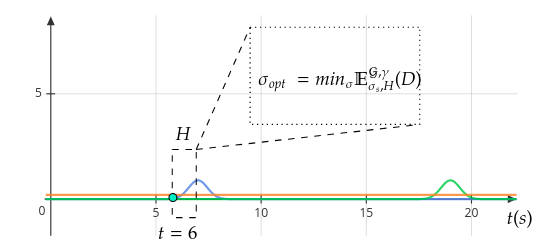
\includegraphics[width=0.7\linewidth]{images/realtime}      
      \caption{\ac{MPC} with \textsc{Uppaal} optimization in a 
      horizon $H$ subject to normal and uniform distributions as stochastic perturbations for $t=6$ in a real time simulation.}
      \label{fig:realtime}
    \end{figure}
    
    The goal is to synthetize a safe and optimal $\sigma_{opt}$ 
    strategy for a given \ac{SHG} $\mathcal{G}$, initial configuration
    $\gamma$, safety set $S$, optimization variable $D$, and time 
    horizon $H$. To obtain 
    $\sigma_{opt}$, the tool \textsc{Uppaal Stratego} first a 
    maximally permissive safe strategy $\sigma_{safe}$ is synthetized
    with respect to $S$. Subsequently, $\sigma_{opt}$ is a sub-strategy
    of $\sigma_{safe}$ (i.e, $\forall \gamma \in \mathbb{C}: 
    \sigma_{opt}(\gamma) \subseteq \sigma_{safe}(\gamma)$ that 
    optimize (minimizes or maximizes) $\mathbb{E}^{\mathcal{G},
    \gamma}_{\sigma,H}(D)$. For additive random variables, the 
    optimal sub-strategy of the maximally permissive strategy is 
    deterministic.
    
  \section{Workflow}
  \label{sec:workflow}
    \begin{figure}[!hbt]
      \centering
      

\tikzset{every picture/.style={line width=0.75pt}} %set default line width to 0.75pt        

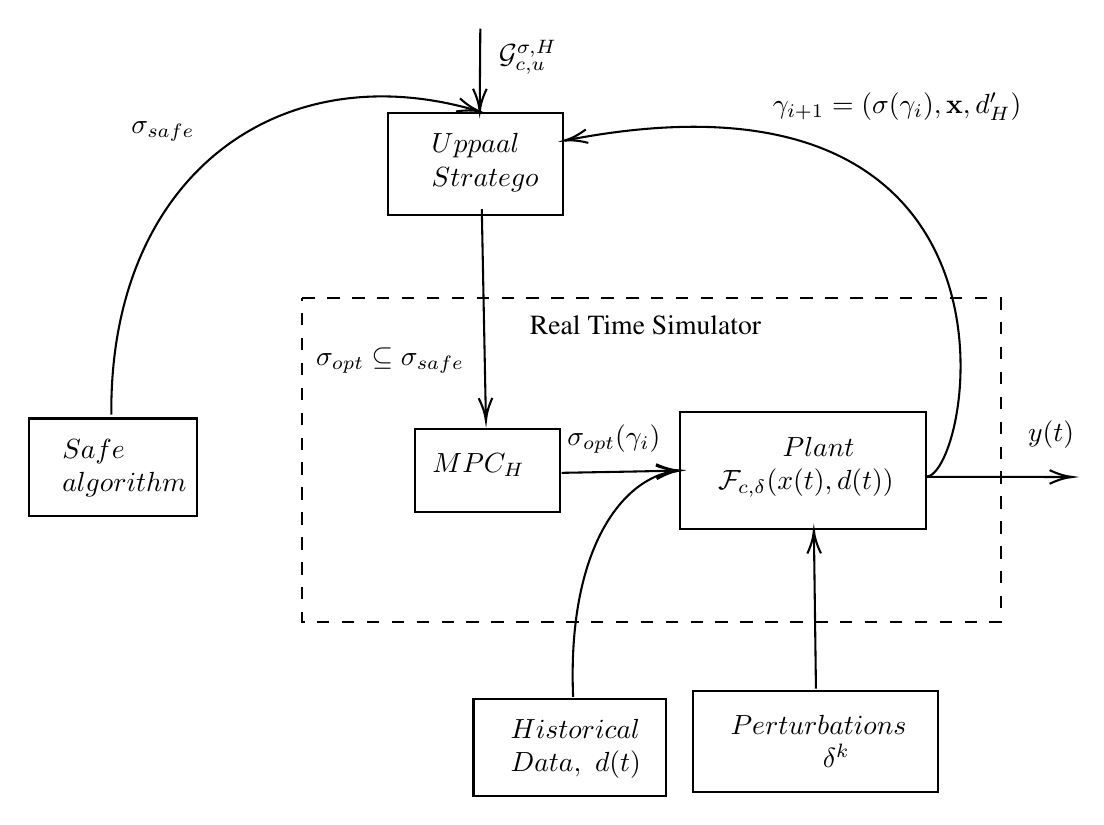
\begin{tikzpicture}[x=0.75pt,y=0.75pt,yscale=-1,xscale=1]
%uncomment if require: \path (0,419); %set diagram left start at 0, and has height of 419

%Shape: Rectangle [id:dp7947774674470398] 
\draw  [dash pattern={on 4.5pt off 4.5pt}] (232.8,147) -- (569.29,147) -- (569.29,303.11) -- (232.8,303.11) -- cycle ;
%Shape: Rectangle [id:dp581005149361487] 
\draw   (274,58) -- (358.29,58) -- (358.29,107.11) -- (274,107.11) -- cycle ;

%Shape: Rectangle [id:dp014468904493361467] 
\draw   (101,205) -- (182.29,205) -- (182.29,252.11) -- (101,252.11) -- cycle ;

%Curve Lines [id:da5102886223745438] 
\draw    (533.29,233.11) .. controls (555.29,233.11) and (593.29,25.11) .. (359.29,71.11) ;
\draw [shift={(359.29,71.11)}, rotate = 348.88] [color={rgb, 255:red, 0; green, 0; blue, 0 }  ][line width=0.75]    (10.93,-3.29) .. controls (6.95,-1.4) and (3.31,-0.3) .. (0,0) .. controls (3.31,0.3) and (6.95,1.4) .. (10.93,3.29)   ;
%Curve Lines [id:da5736171914204411] 
\draw    (140.8,203.2) .. controls (139.8,87.78) and (221.97,28.79) .. (316.86,56.68) ;
\draw [shift={(318.29,57.11)}, rotate = 196.84] [color={rgb, 255:red, 0; green, 0; blue, 0 }  ][line width=0.75]    (10.93,-3.29) .. controls (6.95,-1.4) and (3.31,-0.3) .. (0,0) .. controls (3.31,0.3) and (6.95,1.4) .. (10.93,3.29)   ;
%Straight Lines [id:da7885671872764144] 
\draw    (318.58,17.22) -- (318.3,55.11) ;
\draw [shift={(318.29,57.11)}, rotate = 270.42] [color={rgb, 255:red, 0; green, 0; blue, 0 }  ][line width=0.75]    (10.93,-3.29) .. controls (6.95,-1.4) and (3.31,-0.3) .. (0,0) .. controls (3.31,0.3) and (6.95,1.4) .. (10.93,3.29)   ;
%Shape: Rectangle [id:dp946630032262731] 
\draw   (315.29,340.11) -- (408,340.11) -- (408,387) -- (315.29,387) -- cycle ;

%Shape: Rectangle [id:dp718981269708326] 
\draw   (421,336.11) -- (539.29,336.11) -- (539.29,385.11) -- (421,385.11) -- cycle ;

%Shape: Rectangle [id:dp45733661710220663] 
\draw   (415,202) -- (533.29,202) -- (533.29,258.11) -- (415,258.11) -- cycle ;

%Straight Lines [id:da8932062177607605] 
\draw    (319.29,104.11) -- (321.25,204.11) ;
\draw [shift={(321.29,206.11)}, rotate = 268.88] [color={rgb, 255:red, 0; green, 0; blue, 0 }  ][line width=0.75]    (10.93,-3.29) .. controls (6.95,-1.4) and (3.31,-0.3) .. (0,0) .. controls (3.31,0.3) and (6.95,1.4) .. (10.93,3.29)   ;
%Straight Lines [id:da8287101777047321] 
\draw    (480.29,335.11) -- (479.32,261.11) ;
\draw [shift={(479.29,259.11)}, rotate = 449.25] [color={rgb, 255:red, 0; green, 0; blue, 0 }  ][line width=0.75]    (10.93,-3.29) .. controls (6.95,-1.4) and (3.31,-0.3) .. (0,0) .. controls (3.31,0.3) and (6.95,1.4) .. (10.93,3.29)   ;
%Shape: Rectangle [id:dp34848466006382406] 
\draw   (287,210) -- (357,210) -- (357,250) -- (287,250) -- cycle ;
%Curve Lines [id:da1228487673215457] 
\draw    (363.29,339.11) .. controls (360.36,267.93) and (386.91,233.83) .. (412.34,230.32) ;
\draw [shift={(414.29,230.11)}, rotate = 535.6] [color={rgb, 255:red, 0; green, 0; blue, 0 }  ][line width=0.75]    (10.93,-3.29) .. controls (6.95,-1.4) and (3.31,-0.3) .. (0,0) .. controls (3.31,0.3) and (6.95,1.4) .. (10.93,3.29)   ;
%Straight Lines [id:da8899650593931607] 
\draw    (357.8,231.2) -- (392.81,230.56) -- (412.29,230.15) ;
\draw [shift={(414.29,230.11)}, rotate = 538.79] [color={rgb, 255:red, 0; green, 0; blue, 0 }  ][line width=0.75]    (10.93,-3.29) .. controls (6.95,-1.4) and (3.31,-0.3) .. (0,0) .. controls (3.31,0.3) and (6.95,1.4) .. (10.93,3.29)   ;
%Straight Lines [id:da6729134920451438] 
\draw    (533.29,233.11) -- (601.8,233.2) ;
\draw [shift={(603.8,233.2)}, rotate = 180.07] [color={rgb, 255:red, 0; green, 0; blue, 0 }  ][line width=0.75]    (10.93,-3.29) .. controls (6.95,-1.4) and (3.31,-0.3) .. (0,0) .. controls (3.31,0.3) and (6.95,1.4) .. (10.93,3.29)   ;

% Text Node
\draw (287,64.4) node [anchor=north west][inner sep=0.75pt]    {$ \begin{array}{l}
Uppaal\\
Stratego
\end{array}$};
% Text Node
\draw (109,211.51) node [anchor=north west][inner sep=0.75pt]    {$ \begin{array}{l}
Safe\ \\
algorithm
\end{array}$};
% Text Node
\draw (149,60.4) node [anchor=north west][inner sep=0.75pt]    {$\sigma _{safe}$};
% Text Node
\draw (458,46.4) node [anchor=north west][inner sep=0.75pt]    {$\gamma _{i+1} =( \sigma ( \gamma _{i}) ,\mathbf{x} ,d'_{H})$};
% Text Node
\draw (238,169.4) node [anchor=north west][inner sep=0.75pt]    {$\sigma _{opt} \subseteq \sigma _{safe}$};
% Text Node
\draw (326,21.4) node [anchor=north west][inner sep=0.75pt]    {$\mathcal{G}_{c,u}^{\sigma ,H}$};
% Text Node
\draw (325,346.4) node [anchor=north west][inner sep=0.75pt]    {$ \begin{array}{l}
Historical\ \\
Data,\ d( t)
\end{array}$};
% Text Node
\draw (431,344.4) node [anchor=north west][inner sep=0.75pt]    {$ \begin{array}{l}
Perturbations\\
\ \ \ \ \ \ \ \ \ \ \delta ^{k}
\end{array}$};
% Text Node
\draw (425,210.4) node [anchor=north west][inner sep=0.75pt]    {$ \begin{array}{l}
\ \ \ \ \ \ \ Plant\ \\
\mathcal{F}_{c,\delta }( x( t) ,d( t))
\end{array}$};
% Text Node
\draw (294,220.4) node [anchor=north west][inner sep=0.75pt]    {$MPC_{H}$};
% Text Node
\draw (341,154) node [anchor=north west][inner sep=0.75pt]   [align=left] {{\fontfamily{ptm}\selectfont Real Time Simulator}};
% Text Node
\draw (359,206.4) node [anchor=north west][inner sep=0.75pt]    {$\sigma _{opt}( \gamma _{i})$};
% Text Node
\draw (581,204.4) node [anchor=north west][inner sep=0.75pt]    {$y( t)$};


\end{tikzpicture}

      \captionsetup{format=hang}
      \caption{A general overview about the procedure to control a \ac{SHG}}
      \label{fig:perturbationsgeneration}
    \end{figure}





    
    
    
% \section{Model predictive control for hybrid systems}
% \label{sec:modelpredictivecontroller}
    % Model predictive control \ac{MPC} technique is based on a prediction model 
    % that includes state estimation $x(k)$ through disturbances prediction $d(k)$
    % and also a perturbation distribution(uncertainties) $u(k)$.
    % \begin{gather*} 
    %   x(k+1) = \mathcal{F}_{c,u}(x(k),d(k)), \\
    %   y(k) = x(k), \\
    %   \text{subject to    } h_{c,u}(x(k), d(k)) \leqslant 0
    % \end{gather*}
    % Where $x(k)$, $u(k)$ and $y(k)$ are the state vector, manipulated variables
    % and output vectors at instant  $k$. However, the 
    % control law $c(k) \in \mathbb{C}$, perturbation/uncertainties 
    % $u(k)$ and $x(k)$ as a tuple $\gamma_i=(c, x)$
    %  becomes a configuration and is subject to the switching rule $\sigma(k)$ 
    %  as \autoref{eq:digitalhybridsystem}. 
    % \begin{gather*} 
    %   \pi_{\sigma_T} = \gamma_0::\tau::\gamma_1::\tau::\gamma_2::\tau::\gamma_3::\tau, ...
    % \end{gather*}
    
    % In order to use this model to 
    %  predict the future evolution of the plant from the current state 
    %  $x$, a sequence of $H$ future inputs and perturbations: 

    % From all admissible $\sigma$ combinations, it is chosen the one which
    % provides the best predicted evolution of the plant along a finite 
    % prediction horizon $N$. This is measured by a certain performance index
    % which depends on the considered control objective. In the usual case 
    % of regulation to a given set-point target $y_s$ the performance index 
    % to be minimized penalizes the deviation between the predicted outputs,
    % inputs, perturbances/uncertainties, and corresponding target $y_s$ 
    % respectively as \autoref{eq:costfunction}. The control law is derived from the solution of the optimization problem 
    % by means of the so-called receding horizon technique: At each sampling time
    % $k$, the optimization problem is solved for the current sate $x(k)$,
    % but only the control action corresponding to the current sampling time is 
    % applied, and hence the optimization problem is repeatedly solved. Thus the 
    % control law is given by:
    % \begin{equation} 
    %   \label{eq:costfunction}
    %   c_p = \text{min}_c \norm{x_{pred}(x_0,c,u,d_{pred})-y_s}
    % \end{equation}
    % For each pair $(x(k),c(k))$ in node correspoing to the time $k$ we compute
    % the next $c(k+1)$ in order to have the solution for the next node in time, 
    % in real application the controller strategy computation time 
    % is limited by the switching period $\tau$.
    % \clearpage


        % some definitions are shows as follow:

    % \textbf{Definition 1} \emph{((R,S) - Stability Problem)}. Given a 
    % switched system as shown in figure before, a set of recurrence 
    % ${\mathbb{R}^n}$ and a safe set \emph{S}
    % ${\subset \mathbb{R}^n}$,\textbf{there are} a control rule 
    % ${\sigma : \mathbb{R}^+ \rightarrow U}$ such that, for any
    % initial condition ${x_0  \in  R_1}$ and any perturbation 
    % ${\varpi :\mathbb{R}^+\rightarrow U}$  the
    % following holds:
    
    % \begin{itemize}
    %     \item \emph{ Recurrence in \emph{R}: There are a monotonically 
    %     strictly increasing sequence of (positive) integers
    %     ${\lbrace k_l \rbrace_{l \in \mathbb{N}} , t \in \mathbb{N}}$ such 
    %     that for all ${ l \in \mathbb{N}, \phi(k_l\tau;t_0,x^0,\sigma,w) \in R }$.}
    %     \item \emph{ Stability in \emph{S}: For all ${ t \in \mathbb{R}^n,
    %     \phi(t;t_0,x^0,\sigma,w) \in S}$ .}
    % \end{itemize}
    
    % \textbf{Definition 2} \emph{((${R_1,R_2,S}$) - Reachability )}. %problem
    %     Given a switched system of the form shown above, two sets  
    %     ${ R_1 \subset \mathbb{R}^n}$  and ${ R_2 \subset \mathbb{R}^n}$ 
    %     and a safety set  ${S \subset  \mathbb{R}^n}$, $R_2$ is reachable if
    %     %find a 
    %     there is a control rule  ${\sigma}$ :
    %     ${\mathbb{R}^+\rightarrow U}$ such that, for any initial condition 
    %     ${x_0  \in  R_1}$ and any perturbation  ${\varpi : \mathbb{R}^+  
    %     \rightarrow U}$, the following holds:
    
    % \begin{itemize}
    %     \item  \emph{Reachability from ${R_1}$ to ${R_2}$: there exists 
    %     an integer ${k \in \mathbb{N} }$ such that we have ${ \phi( k_l\tau
    %     ;t_0,x^0,\sigma,w) \in R_2 }$.}
    %     \item \emph{ Stability in S: for all ${ t \in \mathbb{R}^+, 
    %     \phi(t;t_0,x^0,\sigma,w) \in S}$ .}
    % \end{itemize}
    
    


    % defined for all $t \geqslant 0$, where $x(t) \in \mathbb{R}^n$ is the state
    % of the system, $\sigma(.): \mathbb{R}^+ \rightarrow M$ is the switching 
    % rule, and $d(t) \in \mathbb{R}^m$ is the disturbances, the finite
    % set $M= \left\lbrace 1,2,.. N \right\rbrace$ is the set of switching
    % modes of the system. We focus on sampled switched systems: given a sampling
    % period $\tau > 0$, switching will occur at time $\tau, 2\tau, ...$ Switching 
    % depend only on time, and not on states: \emph{this is the main difference with 
    % hybrid system}.

    % We work in the \emph{synchronous} setting for discrete events. This means
    % that all the discrete events are supposed to occur at periodic instants:
    % $\tau, 2\tau, 3\tau, ...$ The switching rule $\sigma(.)$ is thus piecewise
    % constant, we shall consider that $\sigma(.)$ is constant on the time interval
    % $[(k-1)\tau,k\tau[$ for $k \geqslant 1 $. We call \emph{"pattern"} a finite
    % sequence of modes $\pi =  (i_1,i_2,...i_k) \in M^k$. With such a control
    % input, and under a given perturbation $d$, we shall denote by $x(t;t_0;x_0,d,\pi)$
    % the solution at time $t$ of the system.
    
    % \begin{equation} % move to center then
    %     \begin{array}{l}
    %         \dot x (t) = \mathcal{F}_{\sigma(t)}(x(t),d(t)), \\
    %         x(t_0) = x_0, \\
    %         \forall j \in \left\lbrace 1, ... , k \right\rbrace, \sigma(t)=i_j
    %         \in M \text{ for, } t \in \lbrack 1,2 \lbrack
    %     \end{array}
    %     \label{hybridsystem}
    % \end{equation}

    % We will use \ref{hybridsystem} in order to have a clear understanding about
    % some definitions that will be useful for our methodology.

    % \begin{figure}[!h]
    %     \begin{center}
    %         \includegraphics[width=\textwidth*3/5]{images/swiched}
    %         \captionsetup{format=hang}
    %         \caption{Trajectory of a hybrid system. The switching signal
    %         ${\sigma(t)}$ takes on integer values that change at 
    %         discrete-time instances.\citep{liberzon2003switching}}
    %     \end{center}
    % \end{figure}

    % After the system digitalization we can obtain the following:

    % \begin{eqnarray}
    %   \label{eq:digitalhybridsystem}
    %   x(k+1) = f_{\sigma(k)}(x(k),d(k))  \\   
    %   x_0    = x(t_0)
    % \end{eqnarray}

    % It is important to bear in mind the difference between digitalization sampling
    % and period between events or switching in the hybrid system.
